
Results provide three nested layers of evidence for the hallucination-type mechanism.

\subsubsection{5.1 Distributional Evidence: Token Probability Peakedness (h-m1)}

On LLaMA-2-7B TriviaQA (n=488), hallucinated responses show mean peakedness of \textbf{2.936} versus \textbf{2.533} for correct responses (two-sample t-test, p = 0.002). This establishes Step 1 empirically: recall-failure hallucinations produce significantly more peaked token probability distributions, converting the mechanism's distributional assumption into a measured fact for this model and dataset. The Mistral-7B-v0.1 h-m1 run encountered a crash mid-execution; the LLaMA-2-7B result satisfies the must-work gate criterion.

\begin{figure}[htbp]
\centering
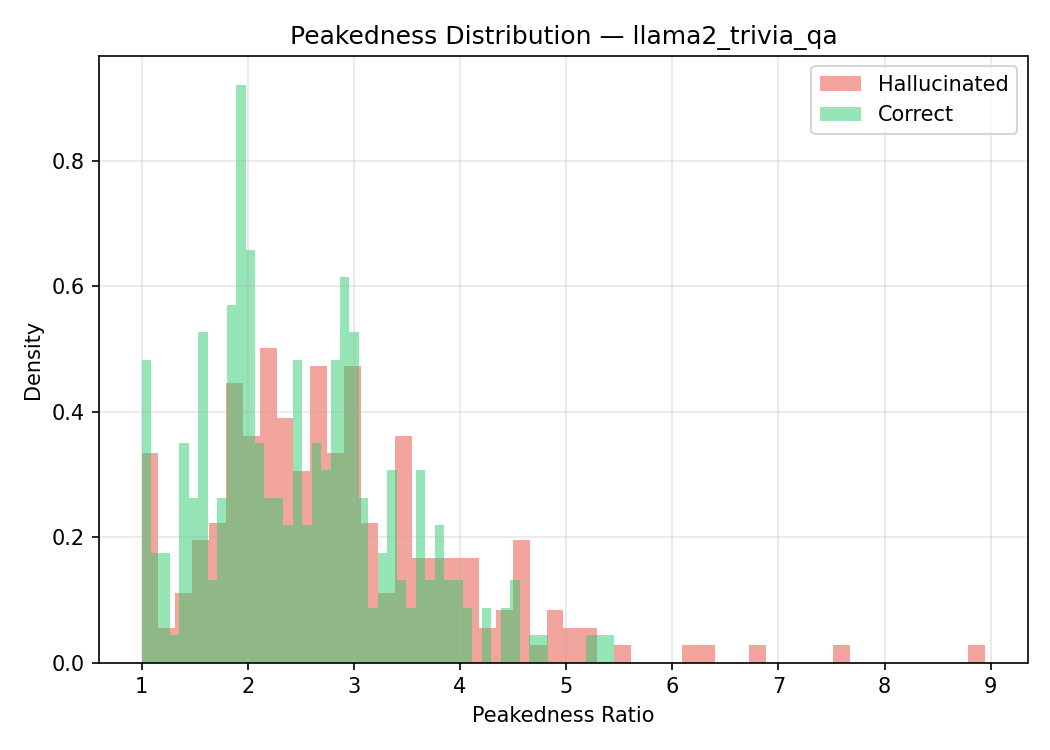
\includegraphics[width=\columnwidth]{figures/peakedness_kde_llama2_trivia_qa.png}
\caption{Peakedness KDE: LLaMA-2-7B, TriviaQA}
\label{fig:peakedness_kde_llama2_trivia_qa}
\end{figure}

\textit{Figure 1. Kernel density estimates of token distribution peakedness for hallucinated (incorrect) vs. correct responses on TriviaQA (LLaMA-2-7B, n=488). Hallucinated responses show a higher-peakedness distribution (mean 2.936 vs. 2.533, p=0.002).}

\subsubsection{5.2 Rank-Correlation Evidence: Aggregation Function Sensitivity (h-m2)}

Spearman rank-correlation between aggregation scores and binary hallucination labels confirms the directional advantage without threshold assumptions. All four (model $\times$ dataset) pairs show the predicted direction; all four bootstrap 95\% confidence intervals exclude zero.

\begin{table*}[htbp]
\centering
\resizebox{\dimexpr 2\columnwidth+\columnsep\relax}{!}{%
\begin{tabular}{lllllll}
\toprule
Model & Dataset & $\rho$(min) & $\rho$(mean) & $\Delta\rho$ ($min-mean)$ & 95\% CI & Direction \\
\midrule
LLaMA-2-7B & TriviaQA (n=488) & 0.604 & 0.397 & **+0.206** & [+0.147, +0.262] & min > mean ✓ \\
Mistral-7B-v0.1 & TriviaQA (n=476) & 0.641 & 0.549 & **+0.092** & [+0.041, +0.143] & min > mean ✓ \\
LLaMA-2-7B & TruthfulQA (n=810) & 0.174 & 0.380 & **$-0.206$** & [$-0.262, -0.147]$ & mean > min ✓ \\
Mistral-7B-v0.1 & TruthfulQA (n=796) & 0.062 & 0.242 & **$-0.180$** & [$-0.237, -0.123]$ & mean > min ✓ \\
\bottomrule
\end{tabular}
}
\end{table*}

The direction reverses cleanly between TriviaQA (min > mean) and TruthfulQA (mean > min), and the reversal is consistent across two architecturally distinct models. Notably, $\rho$(min) on Mistral-7B-v0.1 TruthfulQA is 0.062 (p = 0.080), indicating minimal discrimination for minimum aggregation on flat distributions --- consistent with the mechanism's prediction. Statistical significance (p < 0.05) is met in 7 of 8 individual $\rho$ tests.

\begin{figure}[htbp]
\centering
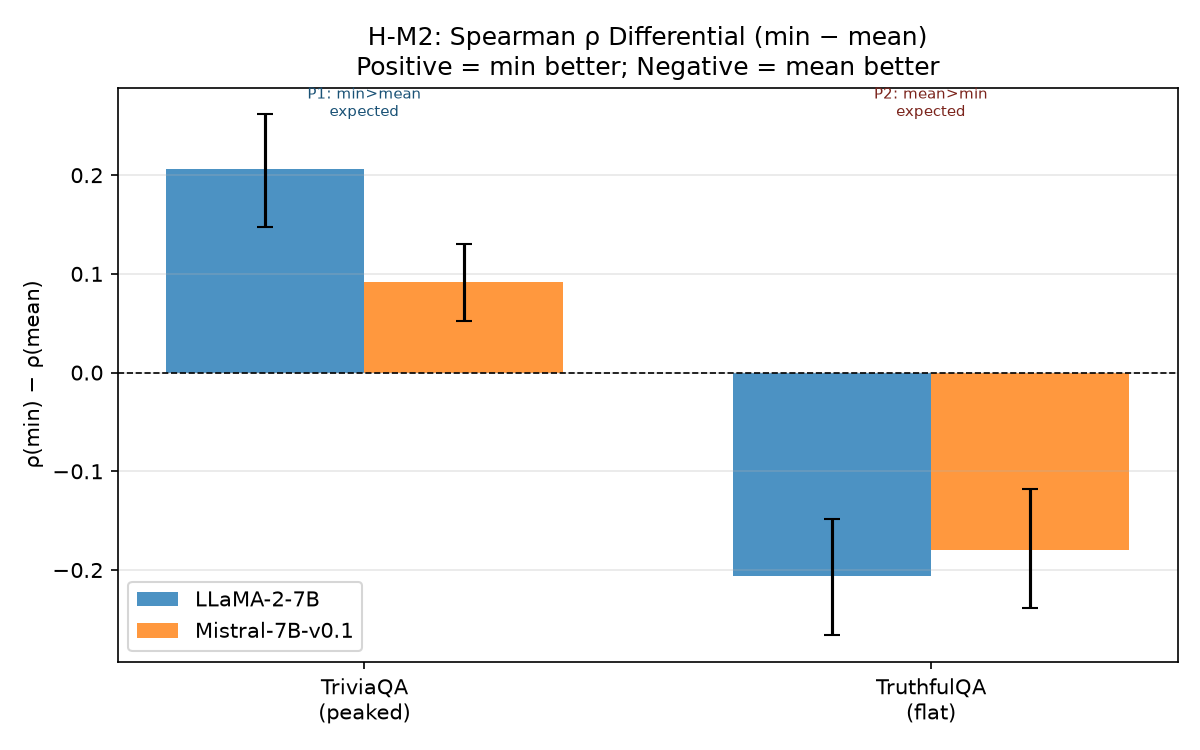
\includegraphics[width=\columnwidth]{figures/rho_differential_bar.png}
\caption{Rank-Correlation Differential Bar Chart}
\label{fig:rho_differential_bar}
\end{figure}

\textit{Figure 2. Spearman $\rho$(min) - $\rho$(mean) with 95\% bootstrap CI error bars for each (model, dataset) pair. Positive values indicate min > mean; negative values indicate mean > min. All four CIs exclude zero.}

\begin{figure}[htbp]
\centering
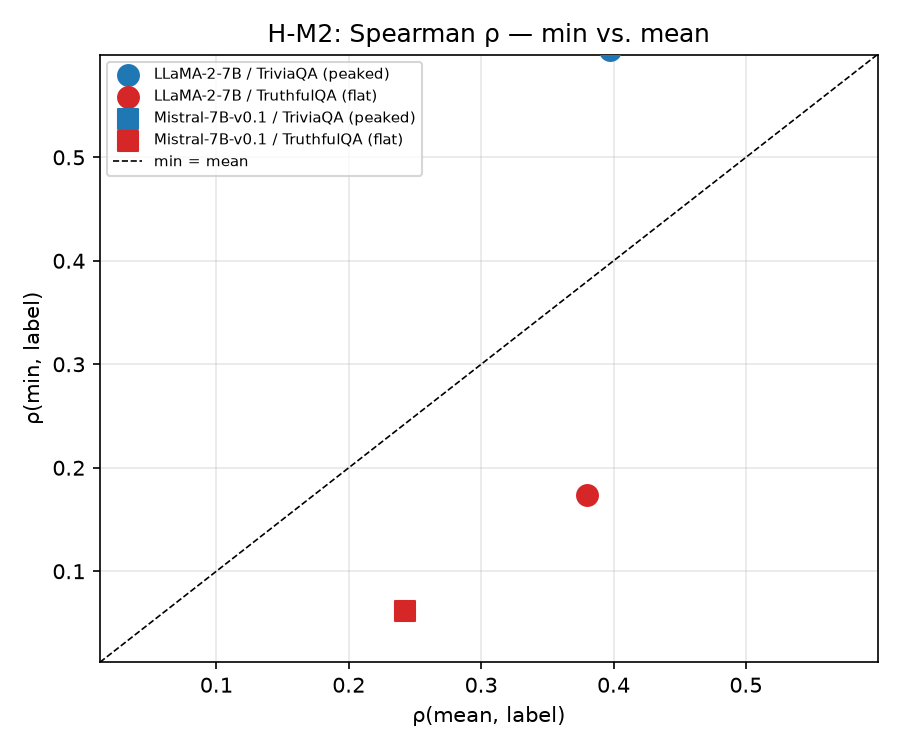
\includegraphics[width=\columnwidth]{figures/rho_scatter.png}
\caption{Rank-Correlation Scatter}
\label{fig:rho_scatter}
\end{figure}

\textit{Figure 3. $\rho$(min) vs. $\rho$(mean) scatter for all (model, dataset) pairs. TriviaQA pairs cluster above the diagonal (min better); TruthfulQA pairs cluster below (mean better).}

\subsubsection{5.3 AUROC Evidence: Threshold-Level Confirmation (h-m3)}

\textbf{Table 1: AUROC with 95\% bootstrap confidence intervals.}

\begin{table*}[htbp]
\centering
\resizebox{\dimexpr 2\columnwidth+\columnsep\relax}{!}{%
\begin{tabular}{lllllllll}
\toprule
Model & Dataset & AUROC(min) & 95\% CI & AUROC(mean) & 95\% CI & AUROC(raw\_sum) & 95\% CI & Best \\
\midrule
LLaMA-2-7B & TriviaQA & 0.849 & [0.815, 0.881] & 0.730 & [0.687, 0.773] & **0.896** & [0.869, 0.921] & raw\_sum \\
LLaMA-2-7B & TruthfulQA & 0.601 & [0.560, 0.639] & **0.721** & [0.686, 0.756] & 0.459 & [0.419, 0.499] & mean \\
Mistral-7B-v0.1 & TriviaQA & 0.892 & [0.862, 0.921] & 0.836 & [0.800, 0.869] & **0.895** & [0.864, 0.921] & raw\_sum \\
Mistral-7B-v0.1 & TruthfulQA & 0.538 & [0.496, 0.581] & **0.649** & [0.608, 0.689] & 0.417 & [0.375, 0.459] & mean \\
\bottomrule
\end{tabular}
}
\end{table*}

\begin{figure}[htbp]
\centering
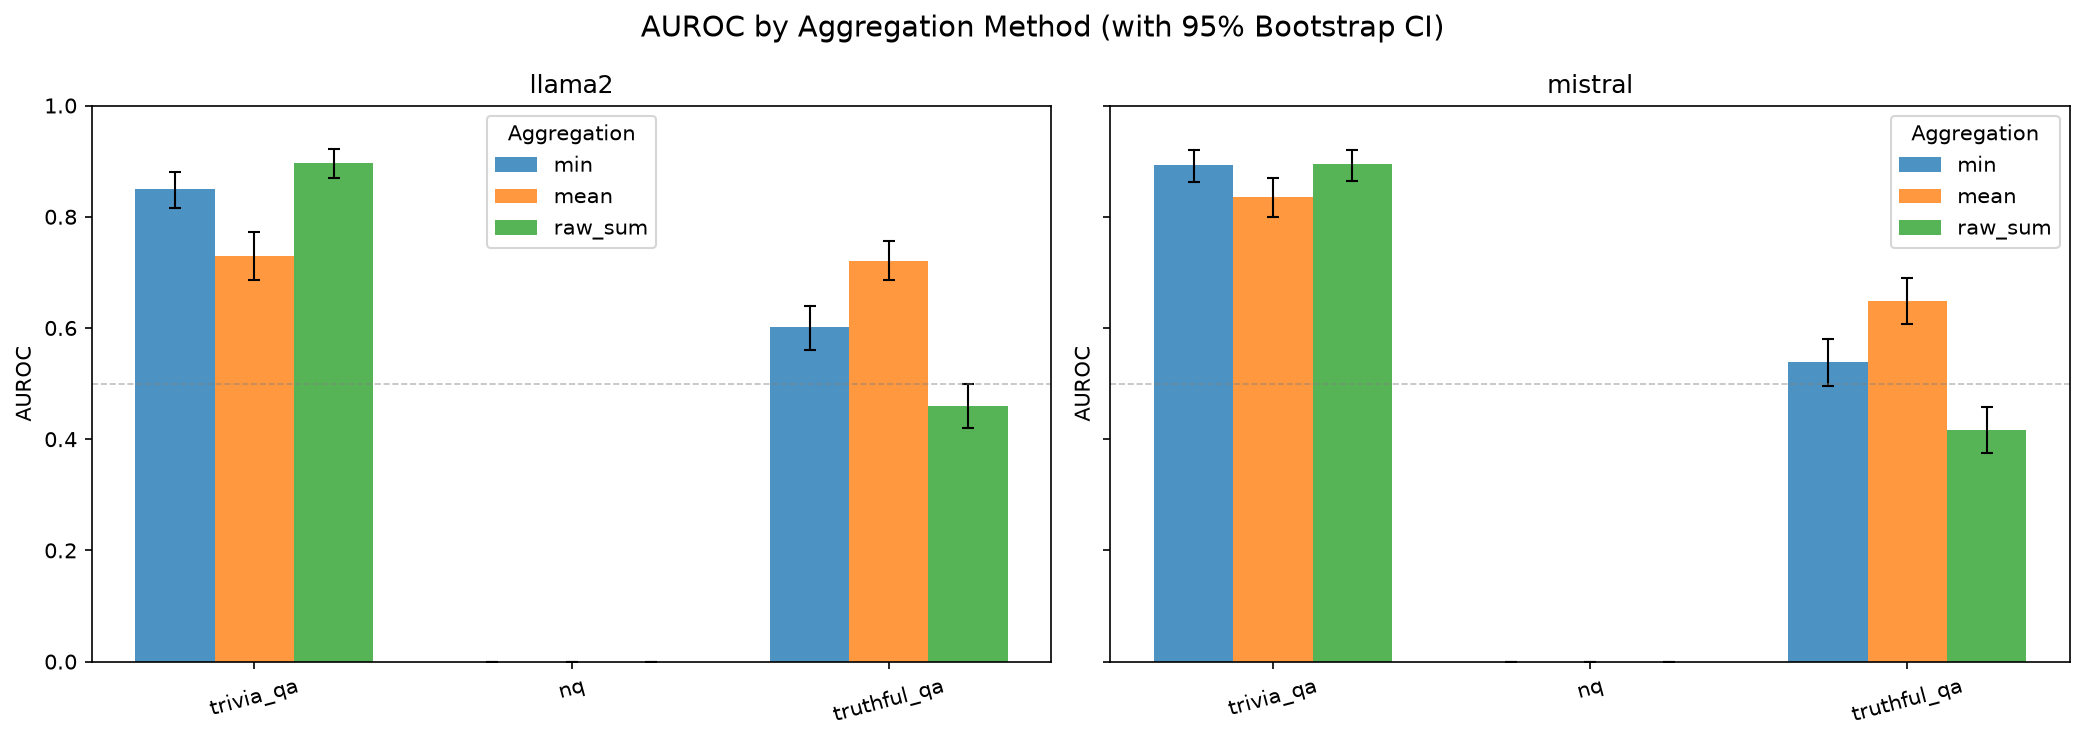
\includegraphics[width=\columnwidth]{figures/fig1_auroc_bar.png}
\caption{AUROC Bar Chart}
\label{fig:fig1_auroc_bar}
\end{figure}

\textit{Figure 4. Grouped bar chart: AUROC(min/mean/raw\_sum) per (model, dataset) with 95\% bootstrap CI error bars. The directional reversal between TriviaQA and TruthfulQA is visible across both models.}

\begin{figure}[htbp]
\centering
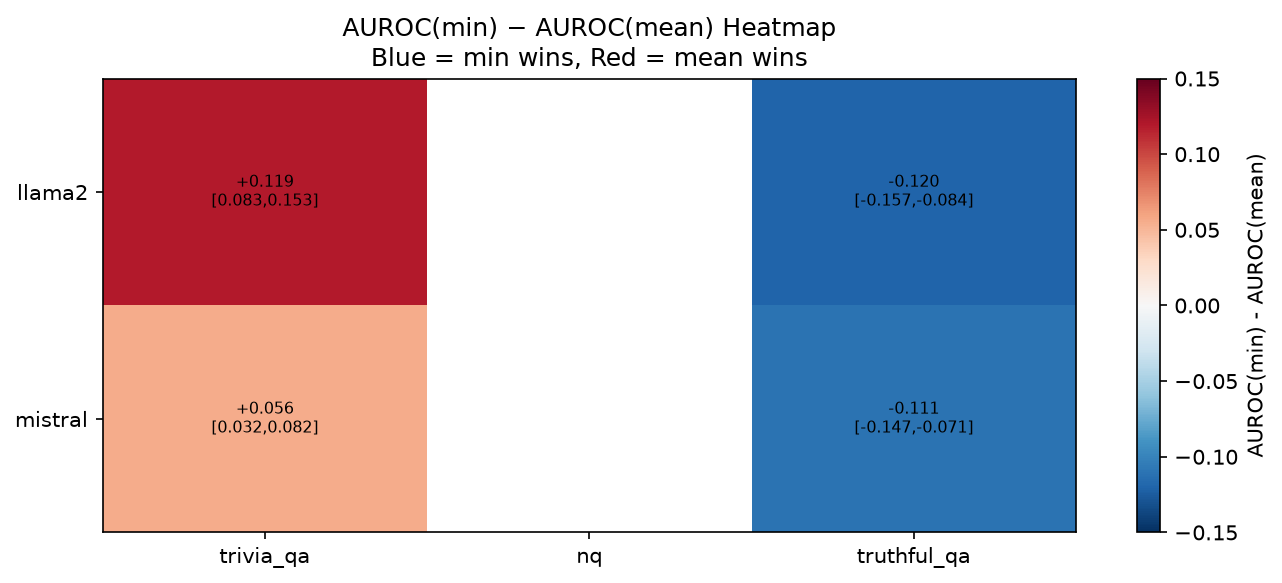
\includegraphics[width=\columnwidth]{figures/fig2_diff_heatmap.png}
\caption{AUROC Differential Heatmap}
\label{fig:fig2_diff_heatmap}
\end{figure}

\textit{Figure 5. Heatmap of AUROC(min) $-$ AUROC(mean) for each (model, dataset) pair. Blue indicates min > mean; red indicates mean > min. The sign reversal between TriviaQA and TruthfulQA is consistent across both models.}

\textbf{P1 (min > mean on TriviaQA):}

\begin{table}[htbp]
\centering
\resizebox{\columnwidth}{!}{%
\begin{tabular}{lll}
\toprule
Model & $\Delta AUROC$ ($min-mean)$ & 95\% CI \\
\midrule
LLaMA-2-7B & **+0.119** & [+0.083, +0.153] \\
Mistral-7B-v0.1 & **+0.056** & [+0.032, +0.082] \\
\bottomrule
\end{tabular}
}
\end{table}

P1 is confirmed for both models on TriviaQA. Effect sizes: 5.6--11.9 AUROC points, with confidence intervals entirely above zero. NQ results are unavailable due to a cache gap (see Section 6.4).

\textbf{P2 (mean > min on TruthfulQA):}

\begin{table}[htbp]
\centering
\resizebox{\columnwidth}{!}{%
\begin{tabular}{lll}
\toprule
Model & $\Delta AUROC$ ($mean-min)$ & 95\% CI \\
\midrule
LLaMA-2-7B & **+0.120** & [+0.084, +0.157] \\
Mistral-7B-v0.1 & **+0.111** & [+0.071, +0.147] \\
\bottomrule
\end{tabular}
}
\end{table}

P2 is confirmed for both models with effect sizes of 11.1--12.0 AUROC points. Both confidence intervals are entirely above zero.

\begin{figure}[htbp]
\centering
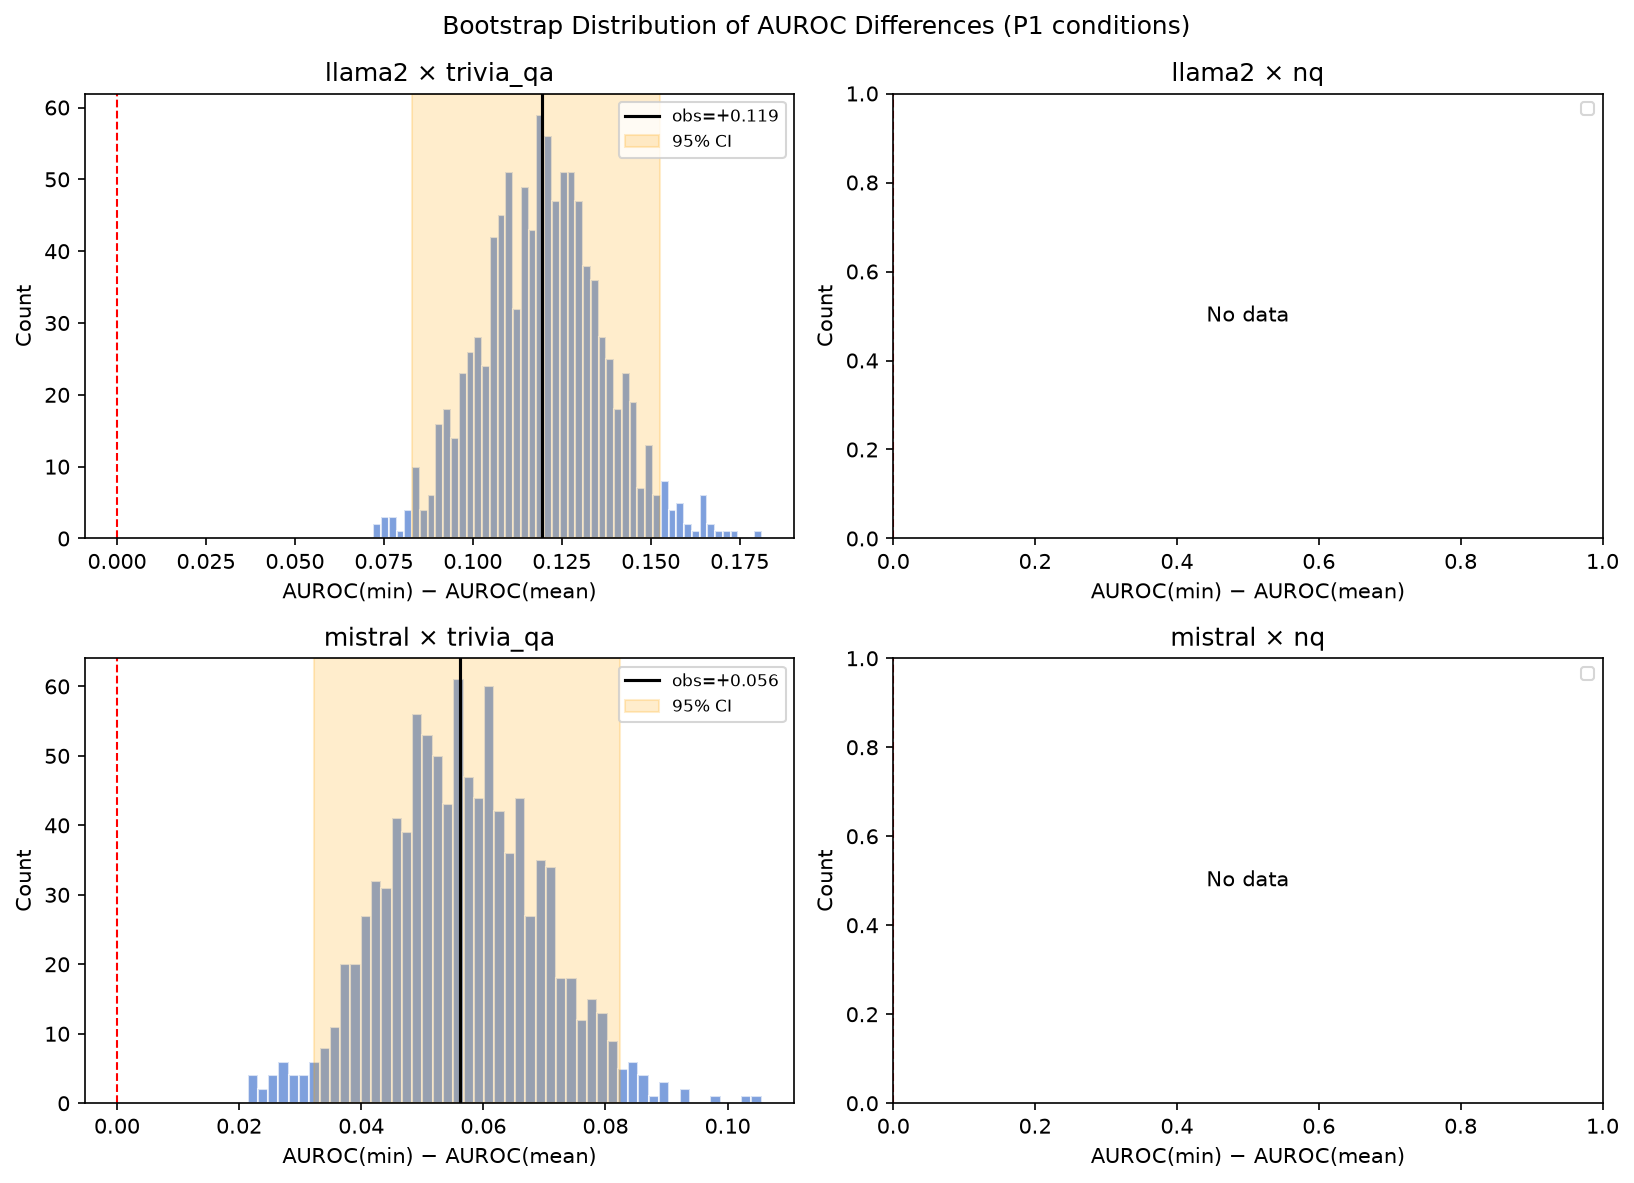
\includegraphics[width=\columnwidth]{figures/fig3_bootstrap_dists.png}
\caption{Bootstrap Differential Distributions}
\label{fig:fig3_bootstrap_dists}
\end{figure}

\textit{Figure 6. Bootstrap distributions of $\Delta AUROC(min-mean)$ for the four P1 conditions (TriviaQA $\times$ 2 models). Distributions are well-separated from zero, confirming statistical reliability.}

\subsubsection{5.4 Unexpected Finding: Raw Sum as Strongest Factual-Recall Detector}

The initial prediction (P3) was that raw unnormalized log-probability sum would be the weakest aggregation due to length bias. This prediction is refuted: raw sum achieves AUROC 0.895--0.896 on TriviaQA --- highest of all three aggregations for both models --- while being the weakest on TruthfulQA (AUROC 0.417--0.459). The contrast between the two benchmark types is approximately 0.44 AUROC for this statistic, the largest single-aggregation gap in the results.

The consistency of raw sum dominance across both model families (identical ranking in both cases) argues against a dataset-specific artifact. The most plausible interpretation is that on factual recall benchmarks, correct answers tend to be longer, with each token assigned high confidence by the model; the unnormalized sum accumulates a larger (more negative) log-probability for correct answers than for shorter or token-uncertain hallucinated answers. A length-stratified AUROC analysis (function implemented in h-e1 codebase but not yet executed) is needed to determine whether the raw sum advantage persists after controlling for answer length.

\begin{figure}[htbp]
\centering
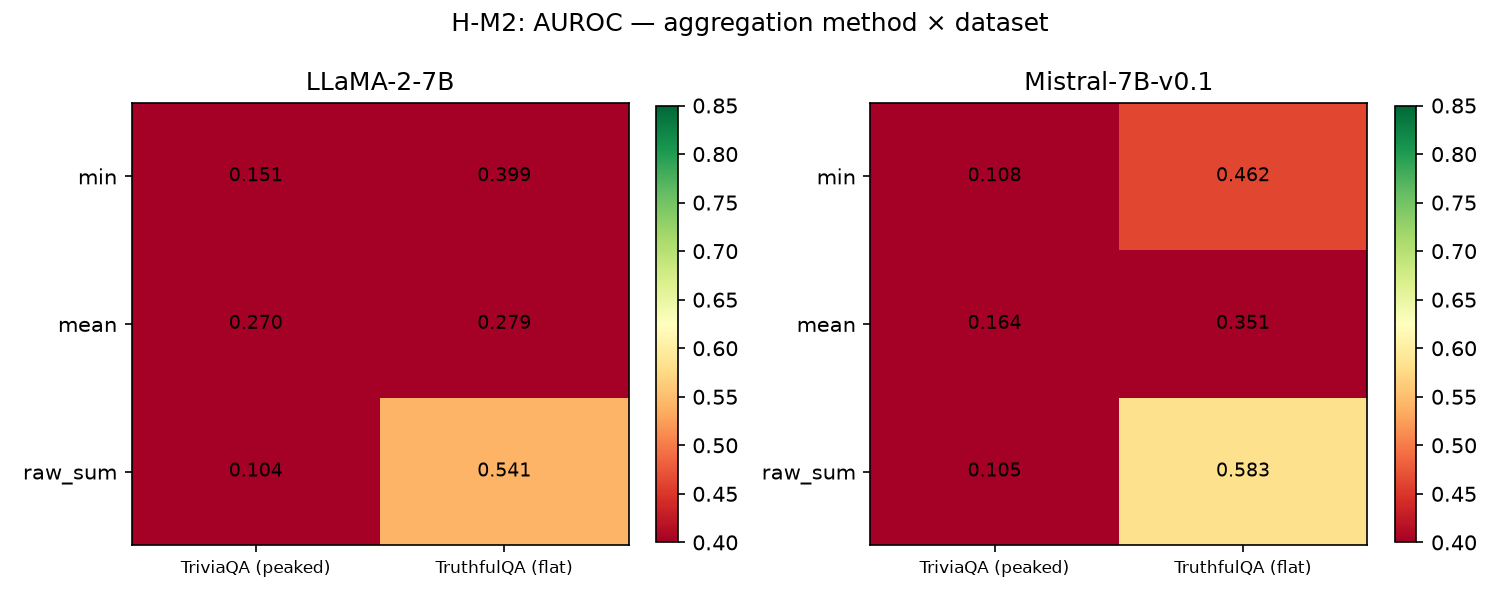
\includegraphics[width=\columnwidth]{figures/auroc_heatmap.png}
\caption{AUROC Heatmap: All Aggregations}
\label{fig:auroc_heatmap}
\end{figure}

\textit{Figure 7. AUROC heatmap: 3 aggregation functions $\times$ 4 (model, dataset) combinations. Raw sum is highest on TriviaQA and lowest on TruthfulQA; mean is highest on TruthfulQA and second on TriviaQA.}

